\documentclass{article}
\usepackage[utf8]{inputenc}
\usepackage{amsmath}
\usepackage{amssymb}
\usepackage{amsthm}
\usepackage{tikz}
\setlength{\parindent}{0pt}

\newtheorem*{theorem}{Theorem}
\newtheorem*{definition}{Definition}
\newtheorem*{lemma}{Lemma}
\newtheorem*{corollary}{Corollary}
\newtheorem{example}{Example}
\newtheorem*{trick}{Trick}
\newtheorem*{question}{Question}

\title{Lecture 17: Polar Coordinates, Application of Double Integrals}
\author{}
\date{}

\begin{document}
    
\maketitle

\section{Double Integrals in Polar Coordinates}

Recall that in polar coordinates, the position is described by two independent 
variables $r$ and $\theta$, instead of $x$ and $y$. The relation between two 
coordinate systems is
\begin{gather*}
  x = r\cos\theta \\
  y = r\sin\theta \\
\end{gather*}

Since the polar coordinate system is only another way of describing positions of 
two-dimentional points, we can also do double integrals in polar coordinates.

\begin{example}
  Calculate the double integral $\iint_R (1 - x^2 - y^2) dA$ in polar 
  coordinates, where $R = $
  \begin{equation*}
    \begin{cases}
      x^2 + y^2 \leq 1 \\
      x \geq 0 \\
      y \geq 0 \\  
    \end{cases}
  \end{equation*}

  First, we need to figure out how to express $dA$ in polar coordinates. If we 
  look at a small region formed by two small changes $\Delta r$ and 
  $\Delta \theta$, the area of the small region is
  \begin{equation*}
    \begin{split}
      \Delta A &= \frac{1}{2}(r + \Delta r)^2 \Delta \theta - \frac{1}{2}r^2 \Delta \theta \\
               &= r \Delta r \Delta \theta + \frac{1}{2}(\Delta r)^2 \Delta \theta \\
    \end{split}
  \end{equation*}
  With the variable changes approaching 0, the limit of the area of the corresponding region is
  \begin{equation*}
    dA = r dr d\theta
  \end{equation*}

  \begin{question}
    Why in the above limitation we ignore the term 
    $\frac{1}{2}(\Delta r)^2 \Delta \theta$? Is it because this term doesn't 
    have any non-differential factors? Is it because this term has higher order 
    of differential factors?
  \end{question}

  Second, we need to determine the order of integral, i.e. whether we integrate 
  $dr$ first, or we integrate $d\theta$ first. In theory, both orders of 
  integrals work, but in most cases, we choose integrating $dr$ first, and then 
  $d\theta$.

  Third, we need to determine the bounds of the inner and outer integrals, by 
  looking at the region in polar coordinates. Since the order of integral we 
  choose is $dr d\theta$, we need to look at the bounds of the variable $r$ with 
  each possible value of the variable $\theta$, and then look at the range of 
  the variable $\theta$. In this case, the range of $r$ is $[0, 1]$ for any 
  value of $\theta$, and the range of $\theta$ is $[0, \frac{\pi}{2}]$.

  Fourth, we need to figure out the function expression in polar coordinates. We 
  do this by utilizing the definition of the polar coordinates. In this example,
  \begin{equation*}
    \begin{split}
      f(x, y) &= 1 - x^2 - y^2 \\
              &= 1 - (r\cos\theta)^2 - (r\sin\theta)^2 \\
              &= 1 - r^2 \\
    \end{split}
  \end{equation*}

  Combining the above together,
  \begin{equation*}
    \begin{split}
      \iint_R (1 - x^2 - y^2) dA &= \int_0^\frac{\pi}{2} \int_0^1 (1 - r^2) r dr d\theta \\
                                 &= \int_0^\frac{\pi}{2} ((\frac{r^2}{2} - \frac{r^4}{4})|_0^1) d\theta \\
                                 &= \int_0^\frac{\pi}{2} \frac{1}{4} d\theta \\
                                 &= (\frac{\theta}{4})|_0^{\frac{\pi}{2}} \\
                                 &= \frac{\pi}{8} \\
    \end{split}
  \end{equation*}
\end{example}

The reasons why we choose to calculate double integrals in the polar coordinates:
\begin{itemize}
  \item The function expression is easier in the polar coordinates.
  \item The bounds of integrals are easier to express in the polar coordinates.
\end{itemize}

It is not often that we can achieve advantage in both aspects. Usually we get 
benefits in one aspect, with the price of sacrificing the other aspect.

\section{Applications of Double Integrals}

\subsection{Application 1: Summing Function Values over a Region}

To find the area of a region $R$, though we can probably do it by setting up a 
single-variable integral, sometimes it is easier to do it with double integrals.

\begin{equation*}
  S = \iint_R 1 dA
\end{equation*}

To find the mass of a planar object with density $\delta$, which is the mass per 
unit area.
\begin{gather*}
  dm = \delta dA \\
  m = \iint_R \delta dA \\
\end{gather*}

\subsection{Application 2: Find the Average Value of a Function over a Region}

To find the average value of a multivariable function $f$ over a region $R$,
\begin{equation*}
  \bar{f} = \frac{1}{\iint_R 1 dA} \iint_R f \cdot dA
\end{equation*}

To find the weighted average value of a multivariable function $f$ over a region 
$R$ with the weight function $w$,
\begin{equation*}
  \bar{f} = \frac{1}{\iint_R w dA} \iint_R w \cdot f \cdot dA
\end{equation*}

To find the center of mass of a planar object with density $\delta$, supposing 
the position of the center of mass is $(\bar{x}, \bar{y})$,
\begin{gather*}
  \bar{x} = \frac{1}{\iint_R \delta dA}\iint_R x \cdot \delta \cdot dA \\
  \bar{y} = \frac{1}{\iint_R \delta dA}\iint_R y \cdot \delta \cdot dA \\
\end{gather*}

\begin{question}
  Why do the above formulas make sense?
\end{question}

\begin{question}
  Can we calculate the center of mass in the polar coordinates as 
  $(\bar{r}, \bar{\theta})$ using the same way as above?

  It doesn't work. 
  
  Counterexample: A planar disk with the center lies in the origin. You can see 
  the center of mass is $r = 0$, but you can never get this result using the 
  similar calculation as above. The result with the above calculation will be 
  $r > 0$.
\end{question}

\subsection{Application 3: Calculate the Moment of Inertia}

Moment of inertia plays a similar role to mass when it comes to rotational 
motion. Mass indicates how hard it is for an object to impart translation 
motion. Moment of inertia indicates how hard it is for an object to rotate 
around an axis.

Moment of inertia for a point mass:

We know that when a point mass $m$ moves at the velocity $v$, it has kinetic 
energy $E_k = \frac{1}{2}mv^2$. Then for a point mass $m$ at distance $r$ to its 
axis and having angular velocity $\omega$:
\begin{gather*}
  v = \omega r \\
  \begin{split}
    E_k &= \frac{1}{2}mv^2 \\
        &= \frac{1}{2}m(\omega r)^2 \\
        &= \frac{1}{2}mr^2 \omega^2 \\
        &= \frac{1}{2}I \omega^2 \\
  \end{split} \\
  I = mr^2 \\
\end{gather*}

Therefore, for such a point mass, its moment of inertia is $mr^2$.

Moment of inertia for an object with the density $\delta$:

For a small area $dA$ of the object, its moment of inertia is:
\begin{gather*}
  dm = \delta dA \\
  dI = dm r^2 = \delta r^2 dA \\
\end{gather*}

The moment of inertia of the object is the sum of the moment of inertia for 
every area of the object:
\begin{equation*}
  \begin{split}
    I &= \iint_R dI \\
      &= \iint_R \delta r^2 dA \\
  \end{split}
\end{equation*}

\begin{question}
  Why the moment of inertia of an object is the sum of the moment of inertia of 
  every point on the object?
\end{question}

\begin{example}
  Calculate the moment of inertia for a disk of radius $a$ with even density 
  rotating around the origin.

  \begin{tikzpicture}
    [help line/.style={dashed}]
    \draw[->] (-3, 0) -- (3, 0) node[right] {x};
    \draw[->] (0, -3) -- (0, 3) node[right] {y};
    \draw (0, 0) node[below right] {O};
    \draw (0, 0) circle (2);
    \draw (2, 0) node[below right] {a};
  \end{tikzpicture}

  Since the object has even density, we can suppose that its density 
  $\delta = 1$. Then
  \begin{equation*}
    \begin{split}
      I_O &= \iint_R \delta r^2 dA \\
          &= \int_0^{2\pi} \int_0^a r^2 r dr d\theta \\
          &= \int_0^{2\pi} ((\frac{r^4}{4})|_0^a) d\theta \\
          &= \int_0^{2\pi} \frac{a^4}{4} d\theta \\
          &= \frac{a^4\theta}{4}|_0^{2\pi} \\
          &= \frac{\pi a^4}{2} \\
    \end{split}
  \end{equation*}
\end{example}

\begin{example}
  Calculate the moment of inertia for a disk of radius $a$ with even density 
  rotating around a point on the circumference.

  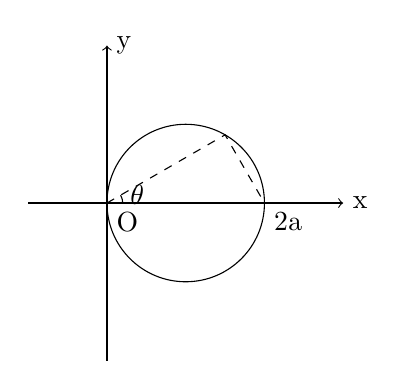
\begin{tikzpicture}
    [help line/.style={dashed}]
    \draw[->] (-1, 0) -- (3, 0) node[right] {x};
    \draw[->] (0, -2) -- (0, 2) node[right] {y};
    \draw (0, 0) node[below right] {O};
    \draw (1, 0) circle (1);
    \draw (2, 0) node[below right] {2a};
    \draw[help line] (0, 0) -- (1.5, 0.866) -- (2, 0);
    \draw (0.2, 0) arc [start angle=0, end angle=30, radius=0.2] node[right] 
      {$\theta$};
  \end{tikzpicture}

  Since the object has even density, we can suppose that its density 
  $\delta = 1$.

  For each possible value of $\theta$, according to the geometric relationship, 
  the bounds of the variable $r$ is $[0, 2a\cos\theta]$. Then
  \begin{equation*}
    \begin{split}
      I_O &= \iint_R \delta r^2 dA \\
          &= \int_{-\frac{\pi}{2}}^{\frac{\pi}{2}} \int_0^{2a\cos\theta} r^2 r dr d\theta \\
          &= \int_{-\frac{\pi}{2}}^{\frac{\pi}{2}} ((\frac{r^4}{4})|_0^{2a\cos\theta}) d\theta \\
          &= \int_{-\frac{\pi}{2}}^{\frac{\pi}{2}} 4a^4\cos^4\theta d\theta \\
          &= 4a^4 \int_{-\frac{\pi}{2}}^{\frac{\pi}{2}} \cos^4\theta d\theta \\
          &= 4a^4 (\frac{3 + 4\cos 2\theta + \cos 4\theta}{8})|_{-\frac{\pi}{2}}^{\frac{\pi}{2}} \\
          &= 4a^4 \frac{3\pi}{8} \\
          &= \frac{3\pi a^4}{2} \\
    \end{split}
  \end{equation*}


\end{example}

\end{document}